\chapter{Технологический раздел}
В данном разеделе представлены требование к ПО, выбор инструментов для реализации и оценки алгоритмов, а также листинги полученного кода.

\section{Требование к ПО}

К программе предъявляется ряд требований:

\begin{itemize}
	\item на вход программа получает количество вершин и матрицу смежностей;
	\item на выходе должен быть получен минимальный путь, проходящий через все вершины графа.
\end{itemize}

\section{Выбор инструментов}
Поскольку наиболее освоенным языком для разработчика является c++, для реализации поставленной задачи был выбран именно он, т.к. таким образом работа будет проделана наиболее быстро и качественно.

Соответственно для компиляции кода будет использоваться компилятор G++.

Чтобы оценить время выполнения программы будет замерятся реальное время, т.к. таким образом можно будет сравнить реализации алгоритмов без и с использованием параллельных вычислений. Для замера реального времени работы программы используется функция clock() т.к. программа тестируется на компьютере с установленной ОС Windows. \cite{clock()}

Кроме этого, необходимо отключить оптимизации компилятора для более честного сравнения алгоритмов. В моём случае это делается с помощью ключа $-O0$ т.к. используется компилятор G++. \cite{gcc_optimization}

\section{Реализация алгоритмов}
На листингах \ref{absolute_find}-\ref{ant2} представлены реализации алгоритма рекурсивного полного перебора и муравьинного алгоритма.

\begin{lstinputlisting}[
	caption={Реализация полного перебора, часть 1},
	label={absolute_find},
	style={c},
	linerange={16-34},
	]{../main.cpp}
\end{lstinputlisting}

\newpage
\begin{lstinputlisting}[
	caption={Реализация полного перебора, часть 2},
	label={absolute_find2},
	style={c},
	linerange={36-63},
	]{../main.cpp}
\end{lstinputlisting}

\newpage
\begin{lstinputlisting}[
	caption={Реализация муравьиного алгоритма, часть 1},
	label={ant1},
	style={c},
	linerange={89-133},
	]{../main.cpp}
\end{lstinputlisting}

\newpage
\begin{lstinputlisting}[
	caption={Реализация муравьиного алгоритма, часть 2},
	label={ant2},
	style={c},
	linerange={134-180},
	]{../main.cpp}
\end{lstinputlisting}

\section{Тестирование}
Тестирование проводилось вручную по методу чёрного ящика.
Результаты представлены на рисунках \ref{test1}-\ref{test2}.

\begin{figure}[h]
	\center{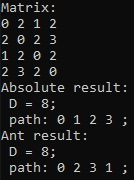
\includegraphics[width=0.3\linewidth]{inc/img/test1}}
	\caption{Результаты тестирования 1}
	\label{test1}
\end{figure}

\begin{figure}[h]
	\center{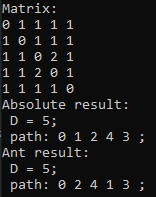
\includegraphics[width=0.3\linewidth]{inc/img/test2}}
	\caption{Результаты тестирования 2}
	\label{test2}
\end{figure}

В обоих тестах пути отличаются, но так как изначально существует несколько путей, оба алгоритма отработали верно.


\section{Вывод}
В данном разделе были выдвинуты требования к ПО, выбраны инструменты реализации выбранных алгоритмов, представлены листинги реализованных алгоритмов, а также проведено тестирование.